\documentclass[10pt, oneside,a4paper]{article}
\usepackage[text={170mm, 230mm}, vmarginratio=1:1]{geometry}
\usepackage[usenames,dvipsnames]{color}
\usepackage{colortbl}
\definecolor{mygray}{gray}{.9}
\usepackage[slantfont,boldfont]{xeCJK}
\setCJKmainfont{SimSun}
\usepackage{array}
\usepackage{tabularx}
\usepackage[colorlinks, linkcolor=black, anchorcolor=blue, citecolor=green]{hyperref}
\usepackage{upgreek}
\usepackage{xcolor, color}
\usepackage[framemethod=tikz]{mdframed}
\usepackage{graphicx, psfrag}
\usepackage{fancyhdr}
\pagestyle{fancy}
\usepackage{indentfirst}
\usepackage{threeparttable}
\usepackage{float}
\linespread{1.5}
\setlength{\parindent}{2em}
\renewcommand{\headrulewidth}{0pt}
\setlength{\headheight}{20 pt}
\hfuzz=\maxdimen
\tolerance=10000
\hbadness=10000
\lhead{}
\chead{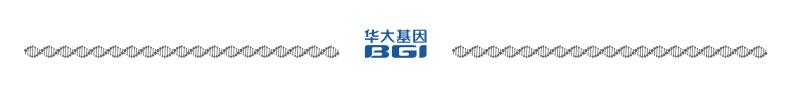
\includegraphics[width=180 mm, keepaspectratio]{./source/bgi_title.jpg}}
\rhead{}
\lfoot{}
\cfoot{\thepage}
\rfoot{}
\begin{document}
\vspace{50 mm}
\title{
\includegraphics[width=80 mm, keepaspectratio]{./source/BGI-LOGO2.png}}
\maketitle
\vspace{30 mm}
\begin{center}
\huge{\textbf {生物信息分析报告}}\par
\vspace{50 mm}
\textbf{\large{华大基因生物技术有限公司}}\par
\end{center}
\newpage
\renewcommand{\contentsname}{目录}
\tableofcontents
\newpage
\section{项目概况}
\vspace{25 mm}
\textbf{\textit{\large{项目名称: }}\large{rice mRNAseq}}\par
\vspace{5 mm}
\textbf{\textit{\large{客户名称: }}\large{yueyao}}\par
\vspace{5 mm}
\textbf{\textit{\large{客户单位: }}\large{华大基因}}\par
\vspace{5 mm}
\textbf{\textit{\large{项目编号: }}\large{000001}}\par
\vspace{5 mm}
\textbf{\textit{\large{物\hspace{2 em}种: }}\large{rice}}\par
\vspace{5 mm}
\textbf{\textit{\large{样本数量: }}\large{EUlef}}\par
\newpage
\section{建库测序流程}
从RNA样品到最终测序数据的分析,样品检测、建库、测序每一个环节都会对数据质量和数量产生影响,而数据质量又会直接影响后续信息分析的结果。
为了从源头上保证测序数据的准确性、可靠性,华大对样品检测、建库、测序每一个生产步骤都严格把控,从根本上确保了高质量数据的产出。流程图如下:
\begin{center}
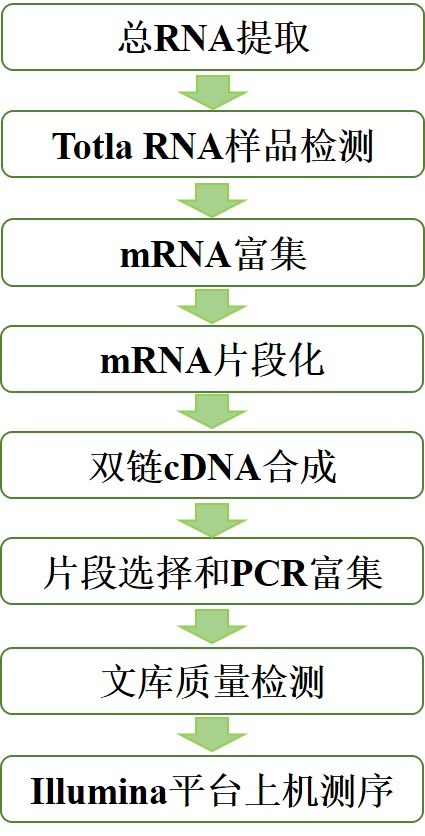
\includegraphics[width=45 mm, keepaspectratio]{./source/library_cst.jpg}
\end{center}
\subsection{Total RNA样品检测}
对RNA样品的检测主要包括4种方法:
\begin{itemize}
\item 琼脂糖凝胶电泳分析RNA降解程度以及是否有污染
\item Nanodrop检测RNA的纯度(OD260/280比值)
\item Qubit对RNA浓度进行精确定量
\item Agilent2100精确检测RNA的完整性
\end{itemize}
\subsection{文库构建}
样品检测合格后,用带有Oligo(dT)的磁珠富集真核生物mRNA(若为原核生物,则通过试剂盒去除rRNA来富集mRNA)。随后加入fragmentation buffer将mRNA打断成短片段,以mRNA为模板,用六碱基随机引物(random hexamers)合成一链cDNA,然后加入缓冲液、dNTPs和DNA polymerase I合成二链 cDNA,随后利用AMPure XP beads纯化双链cDNA。纯化的双链cDNA再进行末端修复、加A尾并连接测序接头,然后用AMPure XP beads进行片段大小选择,最后进行PCR富集得到最终的cDNA文库。构建原理图如下:
\begin{center}
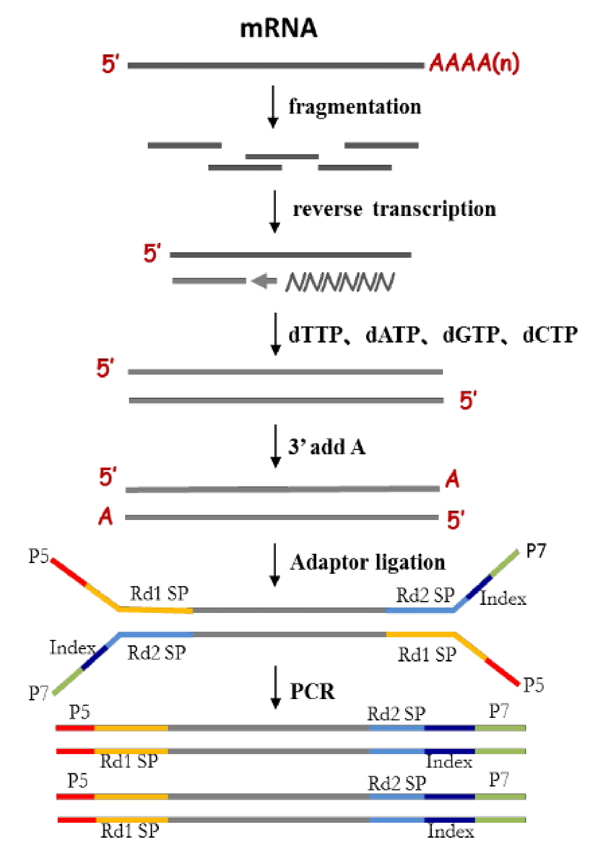
\includegraphics[width=60 mm, keepaspectratio]{./source/library_process.jpg}
\end{center}
\section{生物信息分析流程}
首先对原始下机数据(raw data)进行过滤,将过滤后得到的高质量序列(clean data)比对到该物种的参考基因组上。 
根据比对结果,计算每个基因的表达量。 在此基础上,进一步对样品进行表达差异分析、富集分析和聚类分析。
\begin{center}
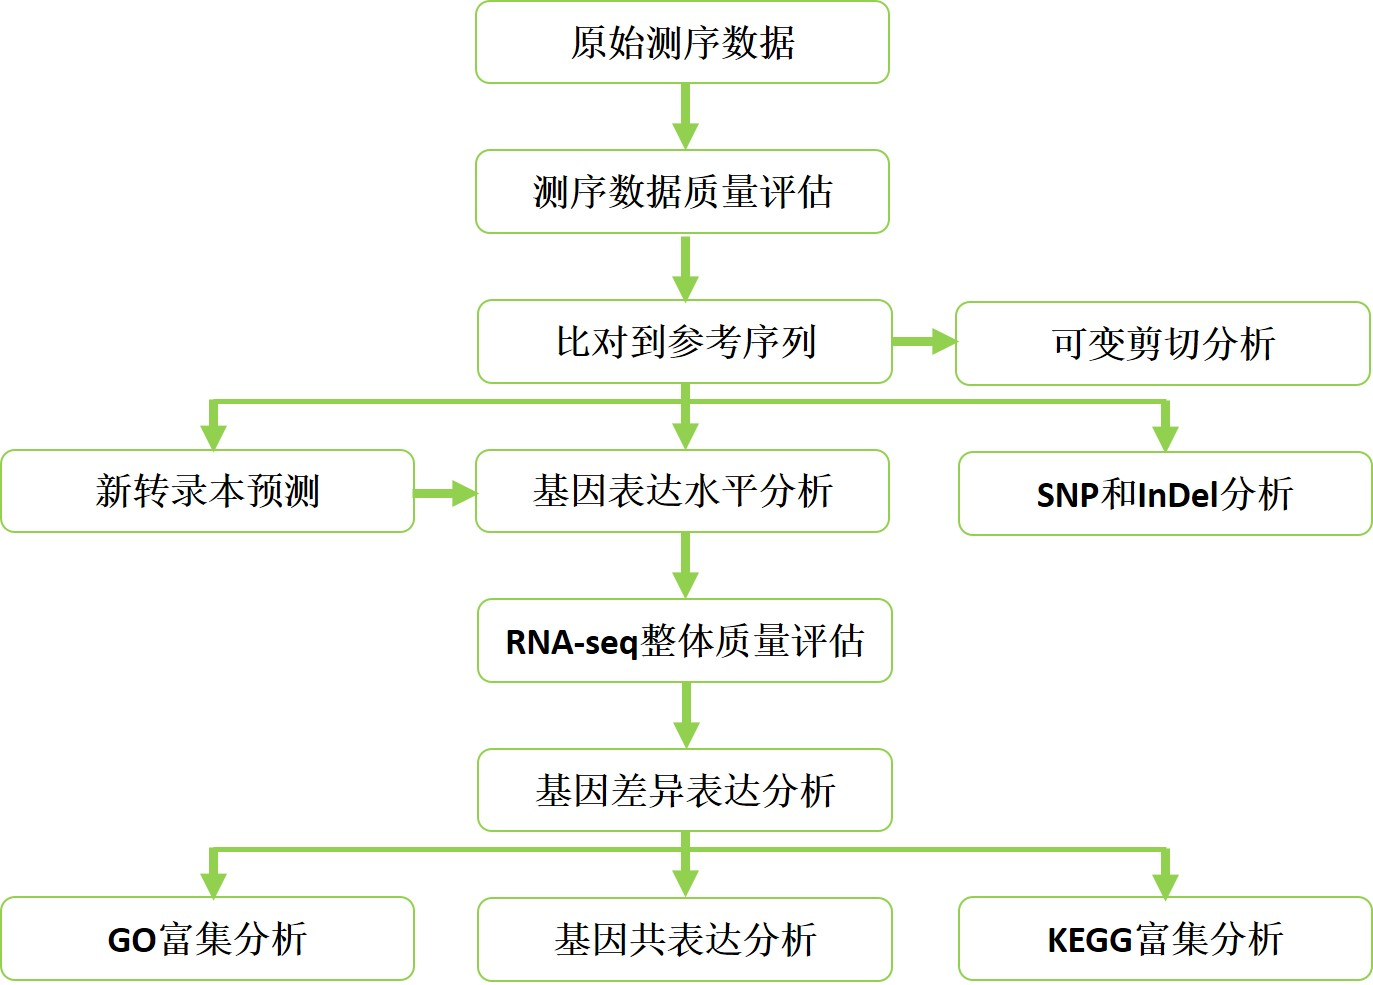
\includegraphics[width=100 mm, keepaspectratio]{./source/als_proc.jpg}
\end{center}
\newpage
\section{结果展示及说明}
\subsection{原始序列数据}
高通量测序 (如Illumina HiSeq$^{TM}$ 2500/Miseq$^{TM}$ )得到的原始图像数据文件经CASAVA碱基识别(Base Calling)分析
转化为原始测序序列(Sequenced Reads),我们称之为Raw Data或Raw Reads,
结果以FASTQ(简称为fq)文件格式存储,其中包含测序序列(reads)的序列信息以及其对应的测序质量信息。\par
FASTQ格式文件中每个read由四行描述,如下:\par
@HWI-ST1276:71:C1162ACXX:1:1101:1208:2458 1:N:0:CGATGT\par
NAAGAACACGTTCGGTCACCTCAGCACACTTGTGAATGTCATGGGATCCAT\par
+\par
\#55???BBBBB?BA@DEEFFCFFHHFFCFFHHHHHHHFAE0ECFFD/AEHH\par
其中第一行以'@'开头,随后为Illumina测序标识符(Sequence Identifiers)和描述文字(选择性部分);\par
第二行是碱基序列;\par
第三行以'+'开头,随后为Illumina测序标识符(选择性部分);\par
第四行是对应碱基的测序质量,该行中每个字符对应的ASCII值减去33,即为对应第二行碱基的测序质量值。\par
测序样本序列见文件夹$\href{run:./BGI\_result/1.CleanData}{/BGI\_result/1.CleanData}$文件夹\par
\subsection{测序数据质量评估}
\subsubsection{测序错误率分布检查}
每个碱基测序错误率是通过测序 Phred数值 (Phred score, Q phred)通过公式(公式 1 : Qphred = -10$\log_{10}e$)转化得到,
而Phred数值是在碱基识别(Base Calling)过程中通过一种概率模型计算得到,这种模型可以准确地预测碱基判别的错误率。
Phred分值,不正确的碱基识别率,碱基正确识别率以及Q-score的对应关系如下表所显示:\par
illumina Casava 1.8 版本碱基识别与Phred分值之间的简明对应关系\par
\vspace{3 mm}
\begin{center}
\begin{tabularx}{110mm}{cccc}
\hline
\textbf{Phred分值} & \textbf{不正确的碱基识别} & \textbf{碱基正确识别率} & \textbf{Q-Score} \\
\hline
10 & 1/10 & 90\% & Q10 \\
20 & 1/100 & 99\% & Q20 \\
30 & 1/1000 & 99.9\% & Q30 \\
40 & 1/10000 & 99.99\% & Q40 \\
\hline
\end{tabularx}
\end{center}
\vspace{5 mm}
\par
测序错误率与碱基质量有关,受测序仪本身、测序试剂、样品等多个因素共同影响。对于RNA-seq技术,测序错误率分布具有两个特点:\par
(1)测序错误率会随着测序序列(Sequenced Reads)长度的增加而升高,这是由于测序过程中化学试剂的消耗导致的,并且为
illumina高通量测序平台都具有的特征。\par
(2)前6个碱基的位置也会发生较高的测序错误率,而这个长度也正好等于在RNA-seq建库过程中反转录所需要的随机引物的长度。
所以前 6个碱基测序错误率较高的原因为随机引物和RNA模版的不完全结合。\par
\subsubsection{测序数据过滤}
测序得到的原始测序序列,里面含有带接头的、低质量的reads,为了保证信息分析质量,必须对raw reads进行过滤,得到clean reads,
后续分析都基于clean reads。\par
数据处理的步骤如下:\par
(1) 去除带接头(adapter)的reads;\par
(2) 去除N(N表示无法确定碱基信息)的比例大于10\%的reads;\par
(3) 去除低质量reads(质量值sQ <= 5的碱基数占整个read长度的50%以上的reads)\par
过滤后reads的质量指标见表\ref{ReadsStatistic},碱基含量分布以及质量分布见图\ref{ReadsBase}和图\ref{ReadsHeatmap}\par
测序样本序列比对到基因组结果见文件夹$\href{run:./BGI\_result/1.CleanData}{./BGI\_result/1.CleanData}$文件夹\par
\vspace{5 mm}
\begin{table}[h]
\centering
\resizebox{\textwidth}{!}{
\begin{threeparttable}
\centering\caption{过滤后的reads质量统计}\label{ReadsStatistic}
\renewcommand{\tablename}{表}
\begin{tabular}{*{7}c}
\hline
\rowcolor{blue!60}
\textbf{Sample} & \textbf{Total Raw Reads(Mb)} & \textbf{Total Clean Reads(Gb)} & \textbf{Total Clean Bases(Gb)} & \textbf{Clean Reads Q20(\%)} & \textbf{Clean Reads Q30(\%)} & \textbf{Clean Reads Ratio(\%)} \\
\hline
EUlef & 40.99 & 38.76 & 3.49 & 97.19 & 91.36 & 94.56 \\
EUski & 62.29 & 58.65 & 5.28 & 97.03 & 91.02 & 94.16 \\

\hline
\end{tabular}
\begin{tablenotes}
\item[1]Q20: 质量值大于20的碱基数目占总碱基数目的比例.\par
\item[1]Total Clean Reads(Mb): 过滤后的reads数\par
\item[2]Total Clean Bases(Gb): 过滤后的碱基总数\par
\item[3]Clean Reads Q20(\%): 过滤后的reads中质量值大于20的碱基数占总碱基数的百分比\par
\item[4]Clean Reads Q30(\%): 过滤后的reads中质量值大于30的碱基数占总碱基数的百分比\par
\item[5]Clean Reads Ratio(\%): 过滤后的reads的比例\par
\end{tablenotes}
\end{threeparttable}}
\end{table}

\begin{figure}[H]
\centering
\includegraphics[width = 0.6\textwidth,natwidth=576,natheight=360]{./BGI_result/1.CleanData/EUlef.base.png}
\renewcommand{\figurename}{图}
\caption{Clean reads的碱基含量分布图}
\label{ReadsBase}
\end{figure}
X轴代表碱基在read中的位置,Y轴代表此类碱基的含量比例。正常情况下,reads每个位置的碱基含量分布稳定,无AT或GC分离现象。
由于Illumina平台在RNA-Seq测序中,反转录成cDNA时所用的6bp随机引物会引起前6个位置的碱基组成存在偏好性,故图中前6bp碱基比例的波动为正常现象。

\begin{figure}[H]
\centering
\includegraphics[width = 0.6\textwidth,natwidth=576,natheight=360]{./BGI_result/1.CleanData/EUlef.qual.png}
\renewcommand{\figurename}{图}
\caption{Clean reads的碱基质量分布图}
\label{ReadsHeatmap}
\end{figure}
X轴代表碱基在read中的位置,Y轴代表碱基质量值,图中每个点表示此位置达到某一质量值的碱基总数,颜色越深表示数目越多。
碱基质量分布反映了测序reads的准确性,测序仪、测序试剂、样品质量等均能影响碱基质量。正常情况下,reads中的前几个碱基质量值不高,
是因为反转录时随机引物不能很好地结合RNA模板;随着测序长度的增加,高质量碱基的比例会有所提高;
但长度达到一定阈值后,由于测序试剂的消耗,高质量碱基的比例会降低。从整体上看,如果低质量(Quality<20)的碱基比例较低,说明测序质量较好。
\vspace{5 mm}

\subsection{Denovo 组装}
对于无参考基因组的项目, 获得clean reads后,需要对clean reads进行拼接以获取后续分析的参考序列。
我们使用Trinity[1]对clean reads进行组装,将Trinity拼接得到的转录本序列,作为后续分析的参考序列。
取每条基因中最长的转录本作为Unigene,以此进行后续的分析。对转录本及Unigene的长度分别进行统计,结果见
表\ref{TranscriptStatistic},表\ref{UnigeneStatistic},图\ref{UnigeneLength}和图\ref{TransLength}
转录组组装的详细结果见文件夹$\href{run:./BGI\_result/2.Assembly}{./BGI\_result/2.Assembly}$文件夹\par
\begin{table}[H]
\centering
\resizebox{\textwidth}{!}{
\begin{threeparttable}[b]
\caption{拼接长度分布情况一览表}\label{TranscriptStatistic}
\renewcommand{\tablename}{表}
\begin{tabular}{*{9}c}
\hline
\rowcolor{blue!60}
\textbf{Sample} & \textbf{Min Length} & \textbf{Mean Length} & \textbf{Max Length} & \textbf{N50} & \textbf{N70} & \textbf{N90} & \textbf{Total} \\
\hline
Unigenes & 251 & 645 & 8893 & 809 & 481 & 302 & 20354233
 \\
Transcripts & 251 & 709 & 8893 & 963 & 542 & 314 & 25890420
 \\

\hline
\end{tabular}
\begin{tablenotes}
\item [1] {N50/N90的定义为: 将拼接转录本按照长度从长到短排序,累加转录本的长度,到不小于总长50\%/90\%的拼接转录本的长度就是N50/N90}
\end{tablenotes}
\end{threeparttable}}
\end{table}
\par
\vspace{5 mm}

\begin{table}[H]
\centering
\resizebox{\textwidth}{!}{
\begin{threeparttable}[b]
\caption{拼接长度频数分布情况一览表}\label{UnigeneStatistic}
\renewcommand{\tablename}{表}
\begin{tabular}{*{6}c}
\hline
\rowcolor{blue!60}
\textbf{Transcript length interval} & \textbf{200-500bp} & \textbf{500-1kbp} & \textbf{1k-2kb} & \textbf{2kbp} & \textbf{Total} \\
\hline
Number of Unigenes & 18933 & 7769 & 3575 & 1275 & 31552
 \\
Number of transcripts & 20517 & 9135 & 4878 & 1973 & 36503
 \\

\hline
\end{tabular}
\begin{tablenotes}
\item [1] {transcripts表示转录本,unigenes表示Unigene}
\end{tablenotes}
\end{threeparttable}}
\end{table}
\vspace{5 mm}

\begin{figure}[H]
\centering
\includegraphics[width = 0.6\textwidth]{./BGI_result/2.Assembly/All_Unigene_length_distribution.png}
\par
\renewcommand{\figurename}{图}
\caption{Unigene的长度分布图。 }
\label{UnigeneLength}
\end{figure}
\begin{center}
X轴代表Unigene长度, Y轴代表相应Unigene的数目。
\end{center}
\par
\vspace{5 mm}

\begin{figure}[H]
\centering
\includegraphics[width = 0.6\textwidth]{./BGI_result/2.Assembly/All_Transcript_length_distribution.png}
\par
\renewcommand{\figurename}{图}
\caption{Transcript的长度分布图。}
\label{TransLength}
\end{figure}

\begin{center}
X轴代表Transcript长度, Y轴代表相应Transcript的数目。
\end{center}
\vspace{5 mm}

\subsection{Unigene功能注释}
组装完毕后,我们将对组装得到的Unigene进行七大功能数据库注释(NR、NT、GO、KOG、KEGG、SwissPprot和InterPro),注释结果见表\ref{AnnotationStatistic}
\begin{table}[H]
\centering
\resizebox{\textwidth}{!}{
\begin{threeparttable}[b]
\caption{功能注释结果统计}\label{AnnotationStatistic}
\renewcommand{\tablename}{表}
\begin{tabular}{*{10}c}
\hline
\rowcolor{blue!60}
\textbf{Values} & \textbf{Total} & \textbf{Nr} & \textbf{Nt} & \textbf{SwissProt} & \textbf{KEGG} & \textbf{KOG} & \textbf{InterPro} & \textbf{GO} & \textbf{Overall} \\
\hline
    Number & 60,740 & 37,136 & 32,509 & 24,806 & 27,146 & 14,481 & 25,746 & 9,798 & 41,004 \\
Percentage & 100\% & 61.14\% & 53.52\% & 40.84\% & 44.69\% & 23.84\% & 42.39\% & 16.13\% & 67.51\% \\

\hline
\end{tabular}
\begin{tablenotes}
\item [1] {Intersection:被七大数据库中所有数据库注释上的Unigene总数及比例}
\item [2] {Overall:被七大数据库中任意一个数据库注释上的Unigene总数及比例}
\end{tablenotes}
\end{threeparttable}}
\end{table}

\subsubsection{NT和NR注释}
NT是NCBI官方的核酸序列数据库,NR是官方的蛋白序列数据库,具有全面、非冗余的特点,我们将NT、NR数据库分为动物、植物、真菌、细菌等几大类,
并将Unigene序列注释到相应的分类,得到相应的功能注释。Unigene与NT注释部分结果展示见表\ref{NtStatistic},Unigene与NR注释部分结果展示见表\ref{NrStatistic},
NR,NT完整注释结果见文件夹$\href{run:./BGI\_result/3.Annotation}{./BGI\_result/3.Annotation}$\par
\begin{table}[H]
\centering
\resizebox{0.9\textwidth}{!}{
\begin{threeparttable}[b]
\caption{NT功能注释部分结果示例}\label{NtStatistic}
\renewcommand{\tablename}{表}
\begin{tabular}{*{5}c}
\hline
\rowcolor{blue!60}
\textbf{Query\_id} & \textbf{Subject\_id} & \textbf{Align\_length} & \textbf{E\_value} & \textbf{Score}  \\
\hline
CL4308.Contig1\_All & gi|57634409|gb|AC141866.11| & 42 & 2e-06 & 60.0 \\
CL4308.Contig1\_All & gi|147855979|emb|AM445472.2| & 29 & 8e-06 & 58.0 \\
CL4308.Contig1\_All & gi|147854678|emb|AM430380.2| & 29 & 8e-06 & 58.0 \\
CL4308.Contig1\_All & gi|147785102|emb|AM486977.2| & 29 & 8e-06 & 58.0 \\
CL4308.Contig2\_All & gi|57634409|gb|AC141866.11| & 42 & 1e-06 & 60.0 \\

\hline
\end{tabular}
\begin{tablenotes}
\item [1] {Query\_id:Unigne的ID(查询ID)}
\item [2] {Subject\_id:数据库中的序列ID,以”|”分割,第二个域是GenBank ID,第四个域是NT数据库中的序列ID}
\item [3] {Align\_length:比对上的序列长度}
\item [4] {E\_value:比对的期望值,值越小代表比对结果越可信}
\item [5] {Score:比对得分,值越大代表比对结果越可信}
\end{tablenotes}
\end{threeparttable}}
\end{table}

\begin{table}[H]
\centering
\resizebox{0.9\textwidth}{!}{
\begin{threeparttable}[b]
\caption{NR功能注释部分结果示例}\label{NrStatistic}
\renewcommand{\tablename}{表}
\begin{tabular}{*{5}c}
\hline
\rowcolor{blue!60}
\textbf{Query\_id} & \textbf{Subject\_id} & \textbf{Align\_length} & \textbf{E\_value} & \textbf{Score}  \\
\hline
CL4309.Contig1\_All & gi|568881138|ref|XP\_006493446.1| & 91 & 2.25E-30 & 135.191 \\
CL4309.Contig1\_All & gi|567870155|ref|XP\_006427699.1| & 91 & 3.84E-30 & 134.42 \\
CL4309.Contig1\_All & gi|593700811|ref|XP\_007150829.1| & 106 & 1.12E-29 & 132.88 \\
CL4309.Contig1\_All & gi|118489278|gb|ABK96444.1| & 91 & 1.46E-29 & 132.494 \\
CL4309.Contig1\_All & gi|225443215|ref|XP\_002269716.1| & 91 & 9.78E-26 & 119.783 \\

\hline
\end{tabular}
\begin{tablenotes}
\item [1] {Query\_id:Unigne的ID(查询ID)}
\item [2] {Subject\_id:数据库中的序列ID,以”|”分割,第二个域是GenBank ID,第四个域是NR数据库中的序列ID}
\item [3] {Align\_length:比对上的序列长度}
\item [4] {E\_value:比对的期望值,值越小代表比对结果越可信}
\item [5] {Score:比对得分,值越大代表比对结果越可信}
\end{tablenotes}
\end{threeparttable}}
\end{table}

根据NR注释结果,统计Unigene注释上不同物种的比例,并绘制物种分布图,见图\ref{Nrspecies}\par

\begin{figure}[H]
\centering
\includegraphics[width = 0.6\textwidth]{./BGI_result/3.Annotation/species_distribution.png}
\par
\renewcommand{\figurename}{图}
\caption{NR库注释物种分布图}
\label{Nrspecies}
\end{figure}

\subsubsection{KOG注释}
我们将Unigene注释到KOG数据库, 并对比对上KOG数据库25个功能组的Unigene进行分类统
计, KOG注释部分结果示例见表\ref{KOGStatistic}, KOG功能分布统计图见图\ref{KOG}。\par
\begin{table}[H]
\centering
\resizebox{0.9\textwidth}{!}{
\begin{threeparttable}[b]
\caption{KOG部分结果示例}\label{KOGStatistic}
\renewcommand{\tablename}{表}
\begin{tabular}{*{5}c}
\hline
\rowcolor{blue!60}
\textbf{Query\_id} & \textbf{Subject\_id} & \textbf{Align\_length} & \textbf{E\_value} & \textbf{Score}  \\
\hline
CL4310.Contig1\_All & YAR019c & 166 & 2e-12 & 70.9 \\
CL4310.Contig1\_All & ECU02g0550 & 148 & 2e-11 & 67.8 \\
CL4310.Contig1\_All & SA1063\_1 & 179 & 7e-11 & 65.9 \\
CL4310.Contig1\_All & ECU01g0630 & 146 & 2e-10 & 64.7 \\
CL4310.Contig1\_All & CAC1728\_1 & 175 & 5e-10 & 63.2 \\

\hline
\end{tabular}
\begin{tablenotes}
\item [1] {Query\_id:Unigne的ID(查询ID)}
\item [2] {Subject\_id:数据库中的序列ID,以”|”分割,第二个域是GenBank ID,第四个域是NR数据库中的序列ID}
\item [3] {Align\_length:比对上的序列长度}
\item [4] {E\_value:比对的期望值,值越小代表比对结果越可信}
\item [5] {Score:比对得分,值越大代表比对结果越可信}
\end{tablenotes}
\end{threeparttable}}
\end{table}

\begin{figure}[H]
\centering
\includegraphics[width = 0.6\textwidth,natwidth=900,natheight=900]{./BGI_result/3.Annotation/All-Unigene.fa.COG.png}
\par
\renewcommand{\figurename}{图}
\caption{KOG功能分布图}
\label{KOG}
\end{figure}
\begin{center}
X轴代表相应的Unigene数目, Y轴代表KOG功能分类名称。
\end{center}

\subsubsection{GO注释}
我们使用Blast2GO[3]软件将所有比对上NR数据库的Unigene结果注释到GO数据库, 并统计注释到
GO三个方面 生物过程(Biological Process)、 细胞组成(Cellular Component)、 分子功能
(Molecular Function)的分类图。 Unigene GO注释部分结果示例见表\ref{GOStatistic},GO功能分布统计图见图\ref{GO}。\par
GO完整注释结果见文件夹$\href{run:./BGI\_result/3.Annotation}{./BGI\_result/3.Annotation}$\par

\begin{table}[H]
\centering
\resizebox{\textwidth}{!}{
\begin{threeparttable}[b]
\caption{Unigene GO注释部分结果示例}\label{GOStatistic}
\renewcommand{\tablename}{表}
\begin{tabular}{*{4}c}
\hline
\rowcolor{blue!60}
\textbf{Ontology} & \textbf{GO term} & \textbf{Number of Genes} & \textbf{Gene members} \\
\hline
biological\_process & biological adhesion & 1,551 & CL1000.Contig1\_All;... \\
cellular\_component & cell & 23,717 & CL1.Contig2\_All;...\\
molecular\_function & antioxidant activity & 82 & CL1122.Contig1\_All;...\\
\hline
\end{tabular}
\begin{tablenotes}
\item [1] {Ontology:GO的三个大类}
\item [2] {GO term:GO三个大类的下一层级}
\item [3] {Number of Genes:注释上某一GO Term的基因数}
\item [4] {Gene members: 注释上某一GO Term的基因名称, 以“;”分割}
\end{tablenotes}
\end{threeparttable}}
\end{table}

\begin{figure}[H]
\centering
\includegraphics[width = 0.6\textwidth,natwidth=900,natheight=900]{./BGI_result/3.Annotation/All-Unigene.fa.GO.png}
\par
\renewcommand{\figurename}{图}
\caption{GO功能分布图}
\label{GO}
\end{figure}
\begin{center}
X轴代表相应的Unigene数目, Y轴代表GO功能分类名称。
\end{center}

\subsubsection{KEGG注释}
将所有Unigene比对到KEGG数据库, 并统计注释上KEGG数据库level1层级和level2层级的Unigene,
绘制KEGG功能分布统计图,见图\ref{KEGG}。 比对上KEGG数据库的部分表格示例见表\ref{KEGGStatistic}, 完整表格下载见表24。\par
KEGG完整注释结果见文件夹$\href{run:./BGI\_result/3.Annotation}{./BGI\_result/3.Annotation}$\par
\begin{table}[H]
\centering
\resizebox{\textwidth}{!}{
\begin{threeparttable}[b]
\caption{Unigene KEGG注释部分结果示例}\label{KEGGStatistic}
\renewcommand{\tablename}{表}
\begin{tabular}{*{4}c}
\hline
\rowcolor{blue!60}
\textbf{Pathway\_level1} & \textbf{Pathway\_level2} & \textbf{Number of Genes} & \textbf{Genes} \\
\hline
Cellular Processes & Cell growth and death  & 776  & CL1015.Contig3\_All;...\\
Environmental Information Processing  & Membrane transport  & 142  & CL1807.Contig1\_All;...\\
Genetic Information Processing  & Folding, sorting and degradation  & 1,274  & CL101.Contig1\_All;...\\
Human Diseases  & Cancers: Overview  & 3,047  & CL10.Contig2\_All;...\\
\hline
\end{tabular}
\begin{tablenotes}
\item [1] {Pathway\_level1: KEGG第一层级}
\item [2] {Pathway\_level2: KEGG第二层级}
\item [3] {Number of Genes: 注释KEGG的Unigene基因个数}
\item [4] {Genes: 注释上KEGG对应的基因}
\end{tablenotes}
\end{threeparttable}}
\end{table}

\begin{figure}[H]
\centering
\includegraphics[width = 0.6\textwidth,natwidth=900,natheight=900]{./BGI_result/3.Annotation/All-Unigene.fa.KEGG.png}
\par
\renewcommand{\figurename}{图}
\caption{KEGG功能分布图}
\label{KEGG}
\end{figure}
\begin{center}
X轴代表相应的Unigene数目, Y轴代表KEGG功能分类。 将基因根据参与的KEGG代谢通路分为7个分支: 细胞过程
(CellularProcesses)、 环境信息处理(EnvironmentalInformationProcessing)、 遗传信息处理(GeneticInformation
Processing)、 人类疾病(HumanDiseasea)(仅限动物)、 代谢(Metabolism)、 有机系统(OrganismalSystems)、 药物
开发(DrugDevelopment)。
\end{center}

\subsubsection{SwissProt注释}
SwissProt数据库是检查过的、 手工注释的蛋白数据库, 我们将Unigene注释到SwissProt数据库, 以
得到更加高质量的注释结果, 注释结果部分表格见表\ref{SwissprotStatistic}。\par
\begin{table}[H]
\centering
\resizebox{0.9\textwidth}{!}{
\begin{threeparttable}[b]
\caption{Swissprot功能注释部分结果示例}\label{SwissprotStatistic}
\renewcommand{\tablename}{表}
\begin{tabular}{*{5}c}
\hline
\rowcolor{blue!60}
\textbf{Query\_id} & \textbf{Subject\_id} & \textbf{Align\_length} & \textbf{E\_value} & \textbf{Score}  \\
\hline
CL4310.Contig1\_All & sp|O81906|B120\_ARATH & 209 & 5e-74 &  274 \\
CL4310.Contig1\_All & sp|O81833|SD11\_ARATH & 197 & 2e-70 &  262 \\
CL4310.Contig1\_All & sp|O64783|Y1137\_ARATH & 188 & 6e-70 &  260 \\
CL4310.Contig1\_All & sp|Q9LPZ3|Y1141\_ARATH & 239 & 3e-69 &  258 \\
CL4310.Contig1\_All & sp|Q9ZT07|RKS1\_ARATH & 199 & 2e-68 &  255 \\

\hline
\end{tabular}
\begin{tablenotes}
\item [1] {Query\_id:Unigne的ID(查询ID)}
\item [2] {Subject\_id:SwissProt数据库中的序列ID}
\item [3] {Align\_length:比对上的序列长度}
\item [4] {E\_value:比对的期望值,值越小代表比对结果越可信}
\item [5] {Score:比对得分,值越大代表比对结果越可信}
\end{tablenotes}
\end{threeparttable}}
\end{table}
同时, 使用维恩图来展示NR、 KOG、 KEGG、 SwissProt 以及 InterPro的注释结果,见图\ref{vennp}。\par

\begin{figure}[H]
\centering
\includegraphics[width = 0.6\textwidth,natwidth=600,natheight=600]{./BGI_result/3.Annotation/Venny/Annotation.venn.png}
\par
\renewcommand{\figurename}{图}
\caption{NR、 KOG、 KEGG、 SwissProt以及InterPro功能注释维恩图}
\label{vennp}
\end{figure}

\subsection{Unigene的CDS预测}
我们使用TransDecoder软件识别Unigene中的候选编码区域,首先提取最长的开放阅读框,然后通过Blast比对SwissProt数据库
和Hmmscan搜索Pfam蛋白同源序列,从而预测编码区域。预测结果见表\ref{CDSStatistic},预测的 CDS 长度分布见图\ref{cds}\par
CDS详细结果见文件夹$\href{run:./BGI\_result/4.Structure/CDSpredict}{./BGI\_result/4.Structure/CDSpredict}$\par
\begin{table}[H]
\centering
\renewcommand{\tablename}{表}
\resizebox{\textwidth}{!}{
\begin{threeparttable}[b]
\caption{CDS的质量指标}\label{CDSStatistic}
\begin{tabular}{*{8}c}
\hline
\rowcolor{blue!60}
\textbf{Software} & \textbf{Total number} & \textbf{Total length} & \textbf{N50} & \textbf{N90} & \textbf{Max length} & \textbf{Min length} & \textbf{Sequence GC} \\
\hline
Blast & 37003 & 28537023 & 771 & 1143 & 753 & 354 & 46.22 \\
ESTScan & 2884 & 984288 & 341 & 342 & 267 & 219 & 49.09 \\
Overall & 39887 & 29521311 & 740 & 1110 & 714 & 327 & 46.32 \\

\hline
\end{tabular}
\begin{tablenotes}
\item [1] {Total number: CDS数目}
\item [2] {Total length: CDS的总长度}
\item [3] {N 5 0 : 用于衡量序列的连续性, 数值越大说明连续性越好, 计算方法为: 按CDS长度从大到小排序后逐个累加至所有CDS总长度的50\%时, 最后一个累加的数值大小即为N50}
\item [4] {N90: 参考N50}
\item [5] {Max length: 最大长度}
\item [6] {Min length: 最小长度}
\item [7] {GC (\%): 碱基G和C的比例}
\end{tablenotes}
\end{threeparttable}}
\end{table}

\begin{figure}[H]
\centering
\includegraphics[width = 0.6\textwidth,natwidth=900,natheight=630]{./BGI_result/4.Structure/CDSpredict/All-Unigene.cds.length.png}
\par
\renewcommand{\figurename}{图}
\caption{CDS长度分布图}
\label{cds}
\end{figure}
\begin{center}
X轴代表CDS长度, Y轴代表相应CDS的数目。
\end{center}
\vspace{5 mm}

\subsection{Unigene的SSR检测}
根据组装结果, 我们对Unigene的 SSR 进行检测,同时为每个 SSR 设计引物。 SSR 长度特征见表\ref{ssrstatic}和图\ref{ssr}。 引物设计结果见表\ref{ssrprimer}。\par
SSR详细结果见文件夹$\href{run:./BGI\_result/4.Structure/SSR}{./BGI\_result/4.Structure/SSR}$\par
\begin{table}[H]
\centering
\renewcommand{\tablename}{表}
\resizebox{\textwidth}{!}{
\begin{threeparttable}[b]
\caption{SSR长度统计}\label{ssrstatic}
\begin{tabular}{*{7}c}
\hline
\rowcolor{blue!60}
\textbf{Number} & \textbf{Mono-nucleotide} & \textbf{Di-nucleotide} & \textbf{Tri-nucleotide} & \textbf{Quad-nucleotide} & \textbf{Penta-nucleotide} & \textbf{Hexa-nucleotide} \\
\hline
4 & 0 & 0 & 0 & 0 & 133 & 358 \\
5 & 0 & 0 & 1,658 & 88 & 25 & 40 \\
6 & 0 & 3,005 & 652 & 18 & 3 & 33 \\
7 & 0 & 1,954 & 358 & 4 & 1 & 4 \\
8 & 0 & 1,457 & 206 & 2 & 4 & 4 \\

\hline
\end{tabular}
\begin{tablenotes}
\item [1] {Number: SSR数目}
\item [2] {Mono-nucleotide: 单碱基重复的SSR数目}
\item [3] {Di-nucleotide: 二碱基重复的SSR数目}
\item [4] {Tri-nucleotide: 三碱基重复的SSR数目}
\item [5] {Quad-nucleotide: 四碱基重复的SSR数目}
\item [6] {Penta-nucleotide: 五碱基重复的SSR数目}
\item [7] {Hexa-nucleotide: 六碱基重复的SSR数目}
\end{tablenotes}
\end{threeparttable}}
\end{table}

\begin{table}[H]
\centering
\renewcommand{\tablename}{表}
\resizebox{\textwidth}{!}{
\begin{threeparttable}[b]
\caption{SSR引物设计表部分结果示例}\label{ssrprimer}
\begin{tabular}{*{5}c}
\hline
\rowcolor{blue!60}
\textbf{Unigene\_ID} & \textbf{FORWARD PRIMER(5'-3')} & \textbf{Tm} & \textbf{REVERSE PRIMER(5'-3')} & \textbf{Tm}  \\
\hline
CL1010.Contig1\_All\_544\_1 & CCTTTTAGATGATCTCCCCAGTT & 59.854 & AAGTCGGAGTCATTCTCTTTCCT & 59.780 \\
CL1010.Contig1\_All\_544\_2 & TCCCCTCTTTCTCTAGCTACCAT & 59.769 & CAAAGATGAAGATGACGAACACA & 60.161 \\
CL1010.Contig1\_All\_544\_3 & CCTTTTAGATGATCTCCCCAGTT & 59.854 & AGTCGGAGTCATTCTCTTTCCTC & 60.253 \\
CL1010.Contig1\_All\_544\_5 & CCTTTTAGATGATCTCCCCAGTT & 59.854 & ACGAACACAGATAAGTCGGAGTC & 59.696 \\
CL1015.Contig1\_All\_548\_1 & TCTTATCTCCTCTTCCACGTTTG & 59.770 & ACCACAGAGACTTATTGGAGCAT & 59.183 \\
CL1015.Contig1\_All\_548\_2 & TCTTATCTCCTCTTCCACGTTTG & 59.770 & TACCACAGAGACTTATTGGAGCA & 58.917 \\

\hline
\end{tabular}
\begin{tablenotes}
\item [1] {Unigene\_ID: 基因ID}
\item [2] {FORWARD PRIMER(5‘-3’): 前端引物序列}
\item [3] {Tm: 前端引物退火温度}
\item [4] {FORWARD PRIMER(5‘-3’): 后端引物序列}
\item [5] {Tm: 后端引物退火温度}
\end{tablenotes}
\end{threeparttable}}
\end{table}

\begin{figure}[H]
\centering
\includegraphics[width = 0.6\textwidth,natwidth=2100,natheight=2100]{./BGI_result/4.Structure/SSR/SSR_statistics.png}
\par
\renewcommand{\figurename}{图}
\caption{SSR长度分布图}
\label{ssr}
\end{figure}
\begin{center}
X轴代表SSR类型, Y轴代表相应的SSR数目
\end{center}

\subsection{SNP检测}
根据组装结果, 我们使用GATK [4]对每个样品进行 SNP 检测, 结果存储为以VCF格式。 SNP 检测结
果见表\ref{snpsum}和图\ref{snp}。\par
SNP详细结果见文件夹$\href{run:./BGI\_result/4.Structure/SNP}{./BGI\_result/4.Structure/SNP}$\par
\begin{table}[H]
\centering
\renewcommand{\tablename}{表}
\resizebox{\textwidth}{!}{
\begin{threeparttable}[b]
\caption{SNP variant type summary}\label{snpsum}
\begin{tabular}{*{10}c}
\hline
\rowcolor{blue!60}
\textbf{Sample} & \textbf{A-G} & \textbf{C-T} & \textbf{Transition} & \textbf{A-C} & \textbf{A-T} & \textbf{C-G} & \textbf{G-T} & \textbf{Transversion} & \textbf{Total} \\
\hline
EUlef & 14499 & 14258 & 28757 & 3695 & 3901 & 3379 & 3860 & 14835 & 43592 \\
EUski & 15547 & 15223 & 30770 & 3935 & 4047 & 3500 & 4054 & 15536 & 46306 \\

\hline
\end{tabular}
\begin{tablenotes}
\item [1] {Sample: 样品名}
\item [2] {A-G: A-G 变异(包括A->G、 G->A)的SNP数目}
\item [3] {C-T: C-T 变异的SNP数目}
\item [4] {Transition: A-G 和 C-T 变异的SNP数目, 嘌呤和嘌呤之间的替换, 或嘧啶和嘧啶之间的替换。}
\item [5] {A-C: A-C 变异的SNP数目}
\item [6] {A-T: A-T 变异的SNP数目}
\item [7] {C-G: C-G 变异的SNP数目}
\item [8] {G-T: G-T变异的SNP数目}
\item [9] {Transversion: A-C,A-T,C-G 和 G-T 变异的SNP数目, 嘌呤和嘧啶之间的替换}
\item [10] {Total: 所有变异类型的总数目}
\end{tablenotes}
\end{threeparttable}}
\end{table}

\begin{figure}[H]
\centering
\includegraphics[width = 0.6\textwidth,natwidth=900,natheight=900]{./BGI_result/4.Structure/SNP/SnpSummary.png}
\par
\renewcommand{\figurename}{图}
\caption{SNP变异类型分布}
\label{snp}
\end{figure}
\begin{center}
X轴代表变异类型, Y轴代表相应的SNP数目
\end{center}


\subsection{Unigene的TF编码能力预测}
做动物、 植物研究的时候, 根据组装结果, 我们对具有编码转录因子( TF )能力的Unigene进行预
测。 我们的项目中, 具有编码转录因子能力的Unigene见表, 同时对预测的转录因子进行家族分类,
见图\ref{tf}。\par
TF详细结果见文件夹$\href{run:./BGI\_result/4.Structure/TFpredict}{./BGI\_result/4.Structure/TFpredict}$\par
\begin{figure}[H]
\centering
\includegraphics[width = 0.6\textwidth,,natwidth=900,natheight=900]{./BGI_result/4.Structure/TFpredict/All-Unigene.TF_family.png}
\par
\renewcommand{\figurename}{图}
\caption{转录因子家族分类}
\label{tf}
\end{figure}
\begin{center}
X轴代表相应的Unigene数目, Y轴代表转录因子家族分类。
\end{center}

\subsection{基因表达量计算}
\subsubsection{基因表达量水平}
根据组装结果, 我们使用 Bowtie2 软件把每个样本的clean reads比对到Unigene, 之后使用 RSEM
计算每个样品的基因表达水平。 比对结果统计表见表\ref{geneexpstat}, 基因表达水平统计表部分结果见表\ref{geneexp}\par
表达量详细结果见文件夹$\href{run:./BGI\_result/5.Quantify/GeneExpression}{./BGI\_result/5.Quantify/GeneExpression}$\par
\begin{table}[H]
\centering
\renewcommand{\tablename}{表}
\resizebox{0.8\textwidth}{!}{
\begin{threeparttable}[b]
\caption{基因表达水平统计表部分结果示例}\label{geneexp}
\begin{tabular}{*{4}c}
\hline
\rowcolor{blue!60}
\textbf{gene\_id} & \textbf{length} & \textbf{expected\_count} & \textbf{FPKM} \\
\hline
CL1.Contig1\_All & 653.00 & 29.01 & 6.40 \\
CL1.Contig2\_All & 450.00 & 6.27 & 2.20 \\
CL10.Contig1\_All & 434.00 & 2.50 & 0.92 \\
CL10.Contig2\_All & 438.00 & 2.50 & 0.91 \\
CL100.Contig1\_All & 827.00 & 53.00 & 8.87 \\

\hline
\end{tabular}
\begin{tablenotes}
\item [1] {gene\_id: Unigene ID}
\item [2] {length: 基因长度}
\item [3] {expected\_count: 基因对应的count值}
\item [4] {FPKM: 基因对应的FPKM值}
\end{tablenotes}
\end{threeparttable}}
\end{table}

\begin{table}[H]
\centering
\renewcommand{\tablename}{表}
\resizebox{\textwidth}{!}{
\begin{threeparttable}[b]
\caption{比对结果统计表}\label{geneexpstat}
\begin{tabular}{*{5}c}
\hline
\rowcolor{blue!60}
\textbf{Sample} & \textbf{Total Bases} & \textbf{Total Reads} & \textbf{Total Mapped Reads} & \textbf{Unique Mapped Reads} \\
\hline
EUlef & 3488310540 & 38759006 & 31255650(80.64\%) & 24294886(62.68\%) \\
EUski & 5278771080 & 58653012 & 48502970(82.69\%) & 38759086(66.08\%) \\

\hline
\end{tabular}
\begin{tablenotes}
\item [1] {Sample: 样品名}
\item [2] {Total Bases: 样品对应的碱基数}
\item [3] {Total Reads: 样品对应的Reads数}
\item [4] {Total Mapped Reads: 所有比对上参考序列的Reads数}
\item [5] {Unique Mapped Reads: 比对到参考序列唯一位置的reads数}
\end{tablenotes}
\end{threeparttable}}
\end{table}

\subsubsection{样品中基因表达量的分布}
根据表达量信息, 本项目采取箱线图展示各样品基因表达水平的分布情况, 可以观察到数据分布的分
散程度, 如图\ref{box}所示。 密度图能够展示样品中基因丰度随着表达量变化的趋势, 可以清晰地反映样本中基
因表达量集中的区间, 如图\ref{dens}所示。 为了更直观地展示每个样品在不同FPKM区间的基因数目, 我们对
FPKM(FPKM<=1、 FPKM1~10、 FPKM>=10)的三种情况进行了基因数目的统计, 如图\ref{exp}所示。\par

\begin{figure}[H]
\centering
\includegraphics[width = 0.6\textwidth,,natwidth=900,natheight=900]{./BGI_result/4.Structure/TFpredict/All-Unigene.TF_family.png}
\par
\renewcommand{\figurename}{图}
\caption{表达量箱线图}
\label{box}
\end{figure}
\begin{center}
X轴为样品名称, Y轴为log10FPKM, 每个区域的箱线图对应五个统计量(自上而下分别为最大值, 上四分位数, 中值,
下四分位数和最小值)。
\end{center}

\begin{figure}[H]
\centering
\includegraphics[width = 0.6\textwidth,,natwidth=900,natheight=900]{./BGI_result/4.Structure/TFpredict/All-Unigene.TF_family.png}
\par
\renewcommand{\figurename}{图}
\caption{表达量密度图}
\label{dens}
\end{figure}
\begin{center}
X轴为log10FPKM, Y轴为基因的密度, 即该表达量下的基因数与表达基因总数的比例
\end{center}

\begin{figure}[H]
\centering
\includegraphics[width = 0.6\textwidth,,natwidth=900,natheight=900]{./BGI_result/4.Structure/TFpredict/All-Unigene.TF_family.png}
\par
\renewcommand{\figurename}{图}
\caption{基因表达量分布图}
\label{exp}
\end{figure}
\begin{center}
X轴表示样品名称, Y轴表示基因数目, 颜色深浅表示不同表达量水平: FPKM<=1的为极低表达水平的基因, FPKM在1
~10之间的为较低表达水平的基因, FPKM>=10为中高表达水平的基因
\end{center}

\subsubsection{PCA分析}
主成分分析(PCA)是将多个变量通过降维为少数几个相互独立的变量(即主成分), 同时尽可能多
地保留原始数据信息的一种多元统计分析方法。 在转录组的分析中, PCA将样本所包含的大量基因表达量
信息降维为少数几个互相无关的主成分, 以进行样本间的比较, 方便找出离群样品、 判别相似性高的样品
簇等。 本项目的PCA分析结果见图\ref{pca}。\par

\begin{figure}[H]
\centering
\includegraphics[width = 0.6\textwidth,,natwidth=900,natheight=900]{./BGI_result/4.Structure/TFpredict/All-Unigene.TF_family.png}
\par
\renewcommand{\figurename}{图}
\caption{PCA分析}
\label{pca}
\end{figure}
\begin{center}
X、 Y轴表示样品表达量经过降维处理后得到的对应主成分的新的数据集, 用来表示样品之间的差距; 坐标轴标签括号
中的数值代表对应主成分解释总体方差的百分比。 点代表每个样品, 同一个颜色代表同一个样品组。
\end{center}


\subsection{时间序列分析}
样品在不同时间阶段一些基因会有相似的表达模式, 根据基因的表达量信息, 可以聚类成与时间相关
联的基因簇, 表达模式一致的基因会被聚到同一个簇, 目前也有文章用该方法分析样品间的组织特异
性。 图\ref{time}显示的是基因聚类成各种基因簇的情况, 同时下载文件中也有每个簇的单个大图供研究人员查
看, 每个基因簇具有的基因详见下表\ref{clus}:\par
表达量详细结果见文件夹$\href{run:./BGI\_result/5.Quantify/GeneExpression}{./BGI\_result/5.Quantify/GeneExpression}$\par
\begin{table}[H]
\centering
\renewcommand{\tablename}{表}
\resizebox{0.8\textwidth}{!}{
\begin{threeparttable}[b]
\caption{基因表达水平统计表部分结果示例}\label{clus}
\begin{tabular}{*{5}c}
\hline
\rowcolor{blue!60}
\textbf{gene\_id} & \textbf{cluster} & \textbf{UHRR1\_fpkm} & \textbf{UHRR2\_fpkm} & \textbf{...} \\
\hline
CL1006.Contig1\_All & 1 & 0 & 0 & ... \\
CL100.Contig3\_All & 1 & 0 & 0 & ... \\
CL1014.Contig3\_All & 1 & 118.28 & 115.68 & ... \\
CL1015.Contig4\_All & 1 & 3.09 & 3.27 & ... \\

\hline
\end{tabular}
\begin{tablenotes}
\item [1] {gene\_id: Unigene ID}
\item [2] {cluster: 基因所对应的基因簇}
\item [3] {Sample1\_fpkm: 各样品基因对应的FPKM值}
\item [4] {Sample2\_fpkm: 各样品基因对应的FPKM值}
\item [5] {...: 其他各个样品基因对应的FPKM值}
\end{tablenotes}
\end{threeparttable}}
\end{table}

\begin{figure}[H]
\centering
\includegraphics[width = 0.6\textwidth,,natwidth=900,natheight=900]{./BGI_result/4.Structure/TFpredict/All-Unigene.TF_family.png}
\par
\renewcommand{\figurename}{图}
\caption{时间序列分析的Mfuzz图}
\label{time}
\end{figure}
\begin{center}
X轴代表各个时间点, Y轴代表均一化后的表达量值
\end{center}

\subsection{差异表达基因检测}
根据各个样品基因表达水平结果, 我们可以检测样品(或者样品组)之间的差异表达基因( DEG ), 本项
目使用DEGseq、 DEseq2、 EBseq、 NOIseq 和 PossionDis算法进行 DEG 检测, 差异表达结果如下:\par
差异表达详细结果见文件夹$\href{run:./BGI\_result/5.Quantify/DifferentExpressedGene}{./BGI\_result/5.Quantify/DifferentExpressedGene}$\par
\begin{table}[H]
\centering
\renewcommand{\tablename}{表}
\resizebox{\textwidth}{!}{
\begin{threeparttable}[b]
\caption{差异表达部分结果示例}\label{deg}
\begin{tabular}{*{6}c}
\hline
\rowcolor{blue!60}
\textbf{GeneID} & \textbf{HBRR2-Expression} & \textbf{UHRR2-Expression} & \textbf{log2FoldChange(UHRR2/HBRR2)} & \textbf{FDR} & \textbf{Pvalue} \\
\hline
Unigene28509\_All  & 0.01  & 6,462.36  & 19.30  & 0.00e+00  & 0.00e+00 \\
CL1804.Contig1\_All  & 0.01  & 524.53  & 15.68  & 0.00e+00  & 0.00e+00 \\
Unigene35357\_All  & 0.01  & 453.05  & 15.47  & 0.00e+00  & 0.00e+00 \\
Unigene20863\_All  & 0.01  & 426.05  & 15.38  & 0.00e+00  & 0.00e+00 \\\hline
\end{tabular}
\begin{tablenotes}
\item [1] {GeneID: Unigene ID}
\item [2] {Sample1-Expression: Sample1表达量}
\item [3] {Sample2-Expression: Sample2表达量}
\item [4] {log2FoldChange(样品2/样品1): 经过log2转换后的样品(组)间的差异表达倍数}
\item [5] {FDR: FDR校正后的统计值}
\item [6] {Pvalue: 显著性统计值}
\end{tablenotes}
\end{threeparttable}}
\end{table}

DEG 检测结果见图\ref{degstat}。 同时使用MA plot、 Scatter plot、 heatmap plot和Volcano plot展示 DEG 的
分布, 见图\ref{ma}, 图\ref{sca}, 图\ref{heatmap}和图\ref{vol}\par

\begin{figure}[H]
\centering
\includegraphics[width = 0.6\textwidth,,natwidth=3600,natheight=2700]{./BGI_result/5.Quantify/DifferentExpressedGene/DEG_number_barplot.png}
\par
\renewcommand{\figurename}{图}
\caption{DEG数量统计图}
\label{degstat}
\end{figure}
\begin{center}
X轴代表每组差异比对方案, Y轴代表相应的DEG数目。 红色代表上调的DEG数目, 蓝色代表下调的DEG数目
\end{center}

\begin{figure}[H]
\centering
\includegraphics[width = 0.6\textwidth,,natwidth=900,natheight=900]{./BGI_result/5.Quantify/DifferentExpressedGene/EUlef-VS-EUski.NOIseq_Method.MA-plot.png}
\par
\renewcommand{\figurename}{图}
\caption{DEG的MA-plot分布图}
\label{ma}
\end{figure}
\begin{center}
X轴代表A值(log2转换后的平均表达水平), Y轴代表M值(log2转换后的差异倍数)。 红色代表上调的DEG, 蓝色代表下调
的DEG, 灰色代表非DEG。
\end{center}

\begin{figure}[H]
\centering
\includegraphics[width = 0.6\textwidth,,natwidth=900,natheight=900]{./BGI_result/5.Quantify/DifferentExpressedGene/EUlef-VS-EUski.NOIseq_Method.MA-plot.png}
\par
\renewcommand{\figurename}{图}
\caption{差异对中所有表达基因散点图}
\label{sca}
\end{figure}
\begin{center}
X、 Y坐标轴均取基因表达量的对数值, 蓝色表示下调基因, 红色表示上调基因, 灰色则是非显著差异基因
\end{center}

\begin{figure}[H]
\centering
\includegraphics[width = 0.6\textwidth,,natwidth=900,natheight=900]{./BGI_result/5.Quantify/DifferentExpressedGene/EUlef-VS-EUski.NOIseq_Method.MA-plot.png}
\par
\renewcommand{\figurename}{图}
\caption{差异基因表达量热图}
\label{heatmap}
\end{figure}
\begin{center}
X轴表示不同样品, Y轴表示差异基因, 颜色越深表示表达量越高, 越浅表示表达量越低
\end{center}

\begin{figure}[H]
\centering
\includegraphics[width = 0.6\textwidth,,natwidth=900,natheight=900]{./BGI_result/5.Quantify/DifferentExpressedGene/EUlef-VS-EUski.NOIseq_Method.Volcano-plot.png}
\par
\renewcommand{\figurename}{图}
\caption{DEG的Volcano-plot分布图}
\label{vol}
\end{figure}
\begin{center}
X轴代表log2转换后的差异倍数值, Y轴代表-log10转换后的显著性值。 红色代表上调的DEG, 蓝色代表下调的DEG,
黑色代表非DEG。
\end{center}


\subsection{差异表达基因GO功能分析}
根据差异基因检测结果, 我们对其 Gene Ontology (GO)功能进行分类以及富集分析。 GO分为分子功
能(Molecular Function) 、 细胞组分(Cellular Component)和生物过程(Biological Process)三大功
能类, 我们将对三大功能类进一步分类以及进行富集分析。 GO功能分类结果见图\ref{goa}, GO功能对应的差异
表达基因上下调统计见图\ref{goup}, GO功能富集结果见图\ref{goenrich}。\par
GO富集分析详细结果见文件夹\par
$\href{run:./BGI\_result/5.Quantify/DifferentExpressedGene/Functional\_Enrichment/GO}{./BGI\_result/5.Quantify/DifferentExpressedGene/Functional\_Enrichment/GO}$\par

\begin{figure}[H]
\centering
\includegraphics[width = 0.6\textwidth,,natwidth=900,natheight=900]{./BGI_result/5.Quantify/DifferentExpressedGene/Functional_Enrichment/GO/EUlef-VS-EUski.NOIseq_Method.GO.png}
\par
\renewcommand{\figurename}{图}
\caption{差异基因GO功能分类图}
\label{goa}
\end{figure}
\begin{center}
X轴代表DEG数目, Y轴代表GO功能分类。
\end{center}

\begin{figure}[H]
\centering
\includegraphics[width = 0.6\textwidth,,natwidth=900,natheight=900]{./BGI_result/5.Quantify/DifferentExpressedGene/Functional_Enrichment/GO/EUlef-VS-EUski.NOIseq_Method.GO.png}
\par
\renewcommand{\figurename}{图}
\caption{差异基因上下调GO功能分类图}
\label{goup}
\end{figure}
\begin{center}
X轴代表GO功能分类,Y轴表示对应GO Term上下调基因数目
\end{center}

\begin{figure}[H]
\centering
\includegraphics[width = 0.6\textwidth,,natwidth=900,natheight=900]{./BGI_result/5.Quantify/DifferentExpressedGene/Functional_Enrichment/GO/EUlef-VS-EUski.NOIseq_Method.Molecular_Function.topGO.png}
\par
\renewcommand{\figurename}{图}
\caption{差异基因GO功能富集结果}
\label{goenrich}
\end{figure}
\begin{center}
有向无环图(DirectedAcyclicGraph, DAG)为差异基因GO富集分析结果的图形化展示方式。 图中, 分支代表包含关系,
从上至下所定义的功能范围越来越小, 方框代表的是每个分类富集程度排名前5的GO Term, 并通过包含关系, 将相关
联的GO Term一起展示。 每个节点上展示了该Term的名称及富集分析校正后的p-value, 颜色越深(红)表示pvalue越
小、 富集程度越高。
\end{center}


\subsection{差异表达基因Pathway功能分析}
根据差异基因检测结果, 我们对其进行KEGG生物通路分类以及富集分析。 通路分类结果见图\ref{kegga}, 通
路富集结果见图\ref{keggenrich}。 富集通路对应的差异表达基因上下调见图\ref{keggup}。\par
KEGG富集分析详细结果见文件夹\par
$\href{run:./BGI\_result/5.Quantify/DifferentExpressedGene/Functional\_Enrichment/Pathway}{./BGI\_result/5.Quantify/DifferentExpressedGene/Functional\_Enrichment/Pathway}$\par

\begin{table}[H]
\centering
\renewcommand{\tablename}{表}
\resizebox{\textwidth}{!}{
\begin{threeparttable}[b]
\caption{差异表达部分结果示例}\label{keggex}
\begin{tabular}{*{6}c}
\hline
\rowcolor{blue!60}
\textbf{\#Pathway} & \textbf{HBRR2-VSUHRR2.PossionDis\_Method(10597)} & \textbf{All-Unigene(27624 )} & \textbf{Pvalue} & \textbf{Qvalue} & \textbf{Pathway ID} \\
\hline
Cell adhesion molecules (CAMs)  & 0.01  & 6,462.36  & 19.30  & 0.00e+00  & 0.00e+00 \\
Ribosome  & 0.01  & 524.53  & 15.68  & 0.00e+00  & 0.00e+00 \\
Arrhythmogenic right ventricular cardiomyopathy (ARVC)  & 0.01  & 453.05  & 15.47  & 0.00e+00  & 0.00e+00 \\
ECM-receptor interaction  & 0.01  & 426.05  & 15.38  & 0.00e+00  & 0.00e+00 \\\hline
\end{tabular}
\begin{tablenotes}
\item [1] {\#Pathway: 代谢通路名称}
\item [2] {group\_Method: 注释上某一通路的差异基因个数}
\item [3] {All-Unigene: 注释上某一通路的Unigene个数}
\item [4] {Pvalue: 显著性统计值}
\item [5] {Qvalue: 校正后的pvalue。 qvalue越小, 表示差异越显著}
\item [6] {Pathway ID: 代谢通路ID号}
\end{tablenotes}
\end{threeparttable}}
\end{table}

\begin{figure}[H]
\centering
\includegraphics[width = 0.6\textwidth,,natwidth=900,natheight=900]{./BGI_result/5.Quantify/DifferentExpressedGene/Functional_Enrichment/Pathway/EUlef-VS-EUski.NOIseq_Method.KEGG.png}
\par
\renewcommand{\figurename}{图}
\caption{差异基因Pathway分类图}
\label{kegga}
\end{figure}
\begin{center}
X轴代表相应的Unigene数目, Y轴代表KEGG功能分类。 将基因根据参与的KEGG代谢通路分为7个分支: 细胞过程
(CellularProcesses)、 环境信息处理(EnvironmentalInformationProcessing)、 遗传信息处理(GeneticInformation
Processing)、 人类疾病(HumanDiseasea)(仅限动物)、 代谢(Metabolism)、 有机系统(OrganismalSystems)、 药物
开发(DrugDevelopment)。
\end{center}

\begin{figure}[H]
\centering
\includegraphics[width = 0.6\textwidth,,natwidth=900,natheight=900]{./BGI_result/5.Quantify/DifferentExpressedGene/Functional_Enrichment/Pathway/EUlef-VS-EUski.NOIseq_Method.KEGG.png}
\par
\renewcommand{\figurename}{图}
\caption{差异基因Pathway富集结果气泡图}
\label{keggup}
\end{figure}
\begin{center}
X轴代表富集因子值, Y轴代表通路名称。 颜色代表qvalue(颜色越白值越大, 越蓝值越小), 值越小代表富集结果越显
著。 点的大小代表DEG数目(点越大代表数目越大, 越小代表数目越少)。 RichFactor指的是富集因子值, 是注释上某一
通路的前景值(差异基因个数)、 与注释上某一通路的背景值(所有基因个数)之商, 数据越大, 说明富集结果越明显
\end{center}

\begin{figure}[H]
\centering
\includegraphics[width = 0.6\textwidth,,natwidth=900,natheight=900]{./BGI_result/5.Quantify/DifferentExpressedGene/Functional_Enrichment/Pathway/EUlef-VS-EUski.NOIseq_Method.path.enrichment.png}
\par
\renewcommand{\figurename}{图}
\caption{富集通路差异基因上下调}
\label{keggenrich}
\end{figure}
\begin{center}
X轴表示Pathway条目, Y轴表示对应Pathway条目上下调基因数目。
\end{center}


\subsection{差异基因蛋白互作分析}
我们使用STRING[5]蛋白互作数据库, 对每组差异表达基因进行蛋白互作分析, 构建互作网络图, 我
们抽取可信度最高的前100个关系进行画图, 蛋白互作关系部分结果见表\ref{ppiex}蛋白互作网络见图\ref{ppip}。\par
PPI分析详细结果见文件夹\par
$\href{run:./BGI\_result/5.Quantify/DifferentExpressedGene/PPI}{./BGI\_result/5.Quantify/DifferentExpressedGene/PPI}$\par

\begin{table}[H]
\centering
\renewcommand{\tablename}{表}
\resizebox{0.8\textwidth}{!}{
\begin{threeparttable}[b]
\caption{差异表达基因蛋白互作关系部分结果示例}\label{ppiex}
\begin{tabular}{*{6}c}
\hline
\rowcolor{blue!60}
\textbf{\#Pathway} & \textbf{HBRR2-VSUHRR2.PossionDis\_Method(10597)} & \textbf{All-Unigene(27624 )} & \textbf{Pvalue} & \textbf{Qvalue} & \textbf{Pathway ID} \\
\hline
Cell adhesion molecules (CAMs)  & 0.01  & 6,462.36  & 19.30  & 0.00e+00  & 0.00e+00 \\
Ribosome  & 0.01  & 524.53  & 15.68  & 0.00e+00  & 0.00e+00 \\
Arrhythmogenic right ventricular cardiomyopathy (ARVC)  & 0.01  & 453.05  & 15.47  & 0.00e+00  & 0.00e+00 \\
ECM-receptor interaction  & 0.01  & 426.05  & 15.38  & 0.00e+00  & 0.00e+00 \\\hline
\end{tabular}
\begin{tablenotes}
\item [1] {\#Pathway: 代谢通路名称}
\item [2] {group\_Method: 注释上某一通路的差异基因个数}
\item [3] {All-Unigene: 注释上某一通路的Unigene个数}
\item [4] {Pvalue: 显著性统计值}
\item [5] {Qvalue: 校正后的pvalue。 qvalue越小, 表示差异越显著}
\item [6] {Pathway ID: 代谢通路ID号}
\end{tablenotes}
\end{threeparttable}}
\end{table}

\begin{figure}[H]
\centering
\includegraphics[width = 0.6\textwidth,,natwidth=900,natheight=900]{./BGI_result5.Quantify/DifferentExpressedGene/PPI/EUlef-VS-EUski.test.png}
\par
\renewcommand{\figurename}{图}
\caption{蛋白互作网络图}
\label{ppip}
\end{figure}
\begin{center}
图中红色表示上调, 蓝色表示下调, 圆圈大小表示相互作用的关系的个数, 圆圈越大表示关系越密集
\end{center}


\subsection{植物抗病基因预测}
根据PRG数据库, 对所有Unigene基因进行植物抗病基因分析, 列表如下:\par
PRG分析详细结果见文件夹$\href{run:./BGI\_result/5.Quantify/DifferentExpressedGene/PRG}{./BGI\_result/5.Quantify/DifferentExpressedGene/PRG}$\par
\begin{table}[H]
\centering
\renewcommand{\tablename}{表}
\resizebox{\textwidth}{!}{
\begin{threeparttable}[b]
\caption{植物抗病基因的注释部分结果示例}\label{prgex}
\begin{tabular}{*{7}c}
\hline
\rowcolor{blue!60}
\textbf{gene\_id} & \textbf{PRGID} & \textbf{Name} & \textbf{Species} & \textbf{Class} & \textbf{GenBank\_ID} & \textbf{GenBank\_Locus} \\
\hline
Unigene43208\_All & PRGDB00078803  & Vvi.12916  & Vitis vinifera  & N  & 225452756  & XM\_002283015 \\
Unigene23022\_All & PRGDB00078803  & Vvi.12916  & Vitis vinifera  & N  & 225452756  & XM\_002283015 \\
Unigene27073\_All  & PRGDB00078803  & Vvi.12916  & Vitis vinifera  & N  & 225452756  & XM\_002283015 \\
Unigene24071\_All  & PRGDB00194209  & Pin.5041  & Phytophthora infestans  & N  & 301091447  & XM\_002895863 \\
\hline
\end{tabular}
\begin{tablenotes}
\item [1] {gene\_id: Unigene ID}
\item [2] {PRGID: PRG数据库的登录号}
\item [3] {Name: 比对上的基因名称}
\item [4] {Species: 物种名}
\item [5] {Class: 抗病基因结构域的类型}
\item [6] {GenBank\_ID: GenBank数据库ID}
\item [7] {GenBank\_Locus: GenBank序列名称}
\end{tablenotes}
\end{threeparttable}}
\end{table}


\subsection{真菌致病基因预测}
根据PHI数据库, 对所有Unigene基因进行真菌致病基因分析, 列表如下:\par
PHI分析详细结果见文件夹$\href{run:./BGI\_result/5.Quantify/DifferentExpressedGene/PHI}{./BGI\_result/5.Quantify/DifferentExpressedGene/PHI}$\par

\begin{table}[H]
\centering
\renewcommand{\tablename}{表}
\resizebox{0.8\textwidth}{!}{
\begin{threeparttable}[b]
\caption{真菌致病基因注释部分结果示例}\label{phiex}
\begin{tabular}{*{4}c}
\hline
\rowcolor{blue!60}
\textbf{gene\_id} & \textbf{Identity} & \textbf{Query\_coverage} & \textbf{Function}  \\
\hline
CL1021.Contig2\_All  & 62.07  & 48.6  & PHI:3945|... \\
CL1140.Contig1\_All  & 65.67  & 54.9  & PHI:1658|... \\
CL1140.Contig2\_All  & 65.67  & 55.3  & PHI:1658|... \\
CL1167.Contig1\_All  & 59.07  & 47.1  & PHI:3594|... \\
\hline
\end{tabular}
\begin{tablenotes}
\item [1] {gene\_id: Unigene ID}
\item [2] {Identity: 比对相似度}
\item [3] {Query\_coverage: 比对序列的覆盖度}
\item [4] {Function: PHI数据库功能注释}
\end{tablenotes}
\end{threeparttable}}
\end{table}

\newpage
\section{报告补充说明}
\subsection{文件目录链接}
为方便您查看项目结果文件,华大基因为您提供了结果文件的目录列表,项目结果文件可通过此目录列表查看,点击目
录列表即可弹出相应结果文件夹(注: 请保证mRNA\_denovo\_report.pdf文件夹和BGI\_result文件夹在同一文件夹下)。
\subsection{结果文件}
结果文件解析说明:\par
\vspace{2 mm}
\begin{center}
\begin{tabularx}{130mm}{ccX}
\hline
\textbf{文件格式} & \textbf{电脑系统} & \textbf{查看程序} \\
\hline
*.tar.gz形式的压缩文件 & windows用户 & 使用解压缩软件如WinRAR、7-Zip等 \\
*.gz形式的压缩文件 & windows用户 & 使用解压缩软件如WinRAR、7-Zip等 \\
*.zip形式的压缩文件 & windows用户 & 使用解压缩软件如WinRAR、7-Zip等 \\
\hline
\end{tabularx}
\end{center}
\vspace{5 mm}
\par
结果文件查看说明;\par
\vspace{2 mm}
\begin{center}
\begin{tabularx}{160mm}{cXX}
\hline
\textbf{文件格式} & \textbf{文件说明} & \textbf{查看程序} \\
\hline
*.fasta & 序列文件,fasta格式,一般为基因序列或者基因组序列。因文件一般较大,打开较为困难 & windows 使用高级文本编辑器 PilotEdit, Notepad++等查看。 \\
*.fq/fastq & 序列文件,fastq格式,一般为reads序列;因文件一般较大,打开较为困难。 & windows 使用高级文本编辑器 PilotEdit, Notepad++等查看。 \\
*.xls, *.txt & 结果数据表格文件,文件以制表符(Tab)分隔 & 用Microsoft Excel或文本编辑器打开 \\
*.png, *.jpg & 结果图像文件 & 用户可以使用图片浏览器打开,如photoshop等 \\
*.pdf & 结果图像文件,矢量图,可以放大和缩小而不失真,方便用户查看和编辑处理 & 用户可以使用Adobe Reader或福昕阅读器等打开 \\
\hline
\end{tabularx}
\end{center}


\newpage
\section{参考文献}
\renewcommand\refname{ }
\begin{thebibliography}{20}
\bibitem{ref1}Cock P., et al.(2010). The SangerFASTQ file format forsequences with quality scores, and the Solexa/Illumina FASTQ variants. Nucleic Acids Research, 38(6): 1767-1771.
\bibitem{ref2}Altschul SF, et al.(1990).Basic local alignment search tool.J Mol Biol. 1990 Oct 5;215(3):403-10.
\bibitem{ref3}Conesa A, et al.(2005).Blast2GO: a universal tool forannotation, visualization and analysis in functional genomics research.Bioinformatics. 2005 Sep 15;21(18):3674-6.
\bibitem{ref4}Quevillon E, et al.(2005).InterProScan: protein domains identifier.Nucleic Acids Res. 2005 Jul 1;33(Web Serverissue):W116-20.
\bibitem{ref5}Iseli C, et al.(1999).ESTScan: a program fordetecting, evaluating, and reconstructing potential coding regions in EST sequences.Proc Int Conf Intell Syst Mol Biol. 1999:138-48.
\bibitem{ref6}Thiel T, et al.(2003).Exploiting EST databases for the development and characterization of gene-derived SSR-markers in barley (Hordeum vulgare L.).Theor Appl Genet. 2003
Feb;106(3):411-22.
\bibitem{ref7}UntergrasserA, et al.(2012).Primer3 -newcapabilities and interfaces.Nucl. Acids Res. (2012)40 (15): e115.
\bibitem{ref8}Kim D, et al.(2015).HISAT: a fast spliced alignerwith lowmemory requirements. Nature Methods 2015.
\bibitem{ref9}McKenna A, et al.(2010).The Genome Analysis Toolkit: a MapReduce framework foranalyzing next-generation DNA sequencing data.Genome Res. 2010 Sep;20(9):1297-303.
\bibitem{ref10}Langmead B, et al.(2012).Fast gapped-read alignment with Bowtie 2. Nature Methods. 2012, 9:357-359.
\bibitem{ref11}Li B, et al.(2011).RSEM: accurate transcript quantification from RNA-Seq data with orwithout a reference genome.BMCBioinformatics. 2011 Aug 4;12:323.
\bibitem{ref12}Eisen, M. B., et al. (2001). Clusteranalysis and display of genome-wide expression patterns. Proc Natl Acad Sci USA, (1998)95(25): 14863-8. 2001.29: 1165-1188.
\bibitem{ref13}M. J. L. de Hoon, et al. (2004). Open Source Clustering Software.Bioinformatics, 20(9): 1453-1454.
\bibitem{ref14}Saldanha, A. J. (2004). Java Treeview--extensible visualization of microarray data. Bioinformatics, 20(17): 3246-8.
\bibitem{ref15}GrabherrMG, et al.(2011).Full-length transcriptome assembly from RNA-Seq data without a reference genome. Nat Biotechnol. 2011 May 15;29(7):644-52.
\bibitem{ref16}Pertea G, et al.(2002).TIGRGene Indices clustering tools (TGICL): a software system forfast clustering of large EST datasets.Bioinformatics (2003)19 (5): 651-652.
\end{thebibliography}
\newpage
\section{常见问题}
\newpage
\section{联系方式}
联系我们\par
服务热线:400-706-6615\par
邮  箱:info@bgitechsolutions.com\par
网  址:www.bgitechsolutions.com\par
地  址:广东省深圳市盐田区北山工业区B2栋(邮编:518083)\par
\end{document}
